\chapter{Formalising the ZDRa and Skeletons}
\label{ch:formal}

In this chapter we take a formal view on the \gls{zdra} and skeletons created. The \gls{zcga} has already been semi formalised using weak type theory \cite{wtt}. 

\section{Formal View on ZDRa}
We denote the star character `*' to denote one or many. We remind the reader that '$\mathbf{\Gamma}$' denotes the schematext of a specification.

\begin{defin}
Let $\mathcal{E}$ be a correctly typed expression. \\ Let $\mathcal{D}$ be a correctly typed definition. \\
Where $((\mathcal{Z}@\mathcal{E})$*$|\mathcal{T}$*$|\mathbb{S}$*$) \in \mathcal{E}$ and $(\mathcal{T}$*$|\mathbb{S}$*$) \in \mathcal{D}$\\
Let $\mathcal{ED}$ be the set containing $\mathcal{E}$'s and $\mathcal{D}$'s.
\end{defin}


\begin{table}[H]
\begin{footnotesize}
\begin{tabular}{| l | l | l |}
\hline
\textbf{Instance} & \textbf{Allowed weak types} & \textbf{Annotations} \\
\hline
\hline
precondition &
$\mathcal{ED} \in \mathbf{\Gamma}$ &
\cgatext{\expression{\mathcal{E}}\definition{\mathcal{D}}} \\

postcondition &
$\mathcal{ED} \in \mathbf{\Gamma}$ &
\cgatext{\expression{\mathcal{E}}\definition{\mathcal{D}}} \\

output &
$\mathcal{ED} \in \mathbf{\Gamma}$ &
\cgatext{\expression{\mathcal{E}}\definition{\mathcal{D}}} \\

stateInvariants &
$\mathcal{ED} \in \mathbf{\Gamma}$ &
\cgatext{\expression{\mathcal{E}}\definition{\mathcal{D}}} \\

stateSchema &
$(\mathcal{Z} \& \mathcal{ED}) | \mathcal{Z} \in \mathbf{\Gamma}$ &
$(\cgatext{\declaration{\mathcal{Z}$*$} \& \expression{\mathcal{E}}\definition{\mathcal{D}}}) | \cgatext{\declaration{\mathcal{Z}$*$}}$ \\

theory &
$(\mathcal{Z} \& \mathcal{ED}) | \mathcal{Z} \in \mathbf{\Gamma}$ &
$(\cgatext{\declaration{\mathcal{Z}$*$} \& \expression{\mathcal{E}}\definition{\mathcal{D}}}) | \cgatext{\declaration{\mathcal{Z}$*$}}$\\

changeSchema &
$(\mathcal{Z} \& \mathcal{ED}) | \mathcal{ED} \in \mathbf{\Gamma}$ &
$(\cgatext{\declaration{\mathcal{Z}$*$} \& \expression{\mathcal{E}}\definition{\mathcal{D}}}) | \cgatext{\expression{\mathcal{E}}\definition{\mathcal{D}}}$ \\

totaliseSchema &
$(\mathcal{Z} \& \mathcal{ED}) | \mathcal{ED} \in \mathbf{\Gamma}$ &
$(\cgatext{\declaration{\mathcal{Z}$*$} \& \expression{\mathcal{E}}\definition{\mathcal{D}}}) | \cgatext{\expression{\mathcal{E}}\definition{\mathcal{D}}}$ \\

axiom &
$\mathcal{Z} \& \mathcal{ED} \in \mathbf{\Gamma} $ &
$\cgatext{\declaration{\mathcal{Z}$*$} \& \expression{\mathcal{E}}\definition{\mathcal{D}}}$ \\

outputSchema &
$\mathcal{Z} \& \mathcal{ED} \in \mathbf{\Gamma} $ &
$\cgatext{\declaration{\mathcal{Z}$*$} \& \expression{\mathcal{E}}\definition{\mathcal{D}}}$ \\

initSchema &
$\mathcal{Z} \& \mathcal{ED} \in \mathbf{\Gamma} $ &
$\cgatext{\declaration{\mathcal{Z}$*$} \& \expression{\mathcal{E}}\definition{\mathcal{D}}}$ \\

\hline
\end{tabular}

\end{footnotesize}
\caption{ZCGa annotations allowed in ZDRa instances \label{tab:zcgainzdra}}
\end{table}

Table \ref{tab:zcgainzdra} shows which \gls{zcga} are allowed to be in certain \gls{zdra} instances.

\paragraph{precondition, postcondition, output, stateInvariants.}
These instances can only contain a correctly typed expression or definition within the schematext. There may be one or more expressions or definitions.

\paragraph{stateSchema, theory.}
These instances can only contain one or more correctly typed declaration \emph{and} one or more correctly typed expression and definition or one or more correctly typed declarations.

\paragraph{changeSchema, totalise.}
These instances can only contain one or more correctly typed declaration \emph{and} one or more correctly typed expression and definition or one or more correctly typed expressions or definitions.

\paragraph{axiom, outputSchema, initSchema}
These instances can only contain one or more correctly typed declarations \emph{and} one or more correctly typed expression and definitions.

\subsection{Properties}

Since we have formally outlined the \gls{zdra} in table \ref{tab:zcgainzdra} we can now write some properties about the \gls{zdra} instances and relations.

\begin{thm}
Using table \ref{tab:zcgainzdra}, the initialOf relation only permits the annotations: \\
 $\mathcal{Z} \& \mathcal{ED}, initialOf, (\mathcal{Z} \& \mathcal{ED}) | \mathcal{Z}$.
\end{thm}

\begin{proof}
From table \ref{tab:relationsallowed} (section \ref{subsec:zdrarelations}) we can see the only legal relation for initialOf is `initSchema $\longrightarrow$ stateSchema'. An initSchema can only have the annotation $\mathcal{Z} \& \mathcal{ED}$ and a stateSchema can only have the annotations $(\mathcal{Z} \& \mathcal{ED}) | \mathcal{Z}$ (from table \ref{tab:zcgainzdra}). Since $\longrightarrow$ represents the relation \emph{initialOf} then we get $\mathcal{Z} \& \mathcal{ED}, initialOf, ((\mathcal{Z} \& \mathcal{ED}) | \mathcal{Z})$.
\end{proof}

\begin{thm}
Using table \ref{tab:zcgainzdra}, the allows relation only permits the annotations: \\
$\mathcal{ED}, allows, \mathcal{ED}$.
\end{thm}

\begin{proof}
The allows relation only permits `precondition $\longrightarrow$ postcondition' (table \ref{tab:relationsallowed}). Both a precondition and postcondition have the \gls{zcga} annotations $\mathcal{ED}$. Since $\longrightarrow$ represents the relation. Then the result is $\mathcal{ED}, allows, \mathcal{ED}$.
\end{proof}

\begin{thm}
Using table \ref{tab:zcgainzdra}, the requires relation only permits the annotations:
\begin{itemize}
\item $\mathcal{Z} \& \mathcal{ED}, requires, \mathcal{ED}$
\item $(\mathcal{Z} \& \mathcal{ED}) | \mathcal{ED}, requires, \mathcal{ED}$
\end{itemize}
\end{thm}

\begin{proof}
Using table (table \ref{tab:relationsallowed}) of permitted relations the requires relation has the following syntax:
\begin{enumerate}
\item `outputSchema $\longrightarrow$ precondition'
\item `outputSchema $\longrightarrow$ output', 
\item `changeSchema $\longrightarrow$ precondition', 
\item `changeSchema $\longrightarrow$ postcondition', 
\end{enumerate} 
\begin{itemize}

\item Using the allowed \gls{zcga} annotations in table \ref{tab:zcgainzdra} we can see that an outputSchema contains only $\mathcal{Z} \& \mathcal{ED}$ and a precondition and output both only contain $\mathcal{ED}$ thus 1 and 2 become $\mathcal{Z} \& \mathcal{ED} \longrightarrow \mathcal{ED}$. Since $\longrightarrow$ represents the relation then we end up with $\mathcal{Z} \& \mathcal{ED}, requires, \mathcal{ED}$.

\item The allowed \gls{zcga} annotations for changeSchema are $(\mathcal{Z} \& \mathcal{ED}) | \mathcal{ED}$ and the allowed \gls{zcga} annotations for both precondition and postcondition are $\mathcal{ED}$ therefore we end up with ($(\mathcal{Z} \& \mathcal{ED}) | \mathcal{ED} \longrightarrow \mathcal{ED}$. Again the $\longrightarrow$ represents the relation so the $\longrightarrow$ becomes `requires' and we are left with $(\mathcal{Z} \& \mathcal{ED}) | \mathcal{ED}, requires, \mathcal{ED}$.
\end{itemize}
\end{proof}

\begin{thm}
Using table \ref{tab:zcgainzdra}, the totalises relation only permits the annotations:
\begin{itemize}
\item $(\mathcal{Z} \& \mathcal{ED}) | \mathcal{ED}), totalises, (\mathcal{Z} \& \mathcal{ED}) | \mathcal{ED}$
\item $(\mathcal{Z} \& \mathcal{ED}) | \mathcal{ED}), totalises, \mathcal{Z} \& \mathcal{ED}$
\end{itemize}
\end{thm}

\begin{proof}
Using table (table \ref{tab:relationsallowed}) of permitted relations the totalises relation has the following syntax:
\begin{enumerate}
\item `totaliseSchema $\longrightarrow$ changeSchema'
\item `totaliseSchema $\longrightarrow$ outputSchema'
\item `totaliseSchema $\longrightarrow$ totaliseSchema'
\end{enumerate} 

\begin{itemize}
\item Table \ref{tab:relationsallowed} shows the \gls{zcga} syntax for totaliseSchema and changeSchema is $(\mathcal{Z} \& \mathcal{ED}) | \mathcal{ED})$. Thus the permitted relations would be $(\mathcal{Z} \& \mathcal{ED}) | \mathcal{ED}) \longrightarrow (\mathcal{Z} \& \mathcal{ED}) | \mathcal{ED})$ for points 1 and 3. Since $\longrightarrow$ represents the relation `totalises' in this case we would have $(\mathcal{Z} \& \mathcal{ED}) | \mathcal{ED}), totalises, (\mathcal{Z} \& \mathcal{ED}) | \mathcal{ED})$. Hence the first part of the theorem is proven.

\item Output schema has the \gls{zcga} sytntax $(\mathcal{Z} \& \mathcal{ED})$ according to table \ref{tab:zcgainzdra}. If totaliseSchema has the \gls{zcga} syntax $(\mathcal{Z} \& \mathcal{ED}) | \mathcal{ED})$ then using point 2 the permitted relation would be $(\mathcal{Z} \& \mathcal{ED}) | \mathcal{ED}) \longrightarrow \mathcal{Z} \& \mathcal{ED}$. Again since $\longrightarrow$ represent totalise in this case we conclude with $(\mathcal{Z} \& \mathcal{ED}) | \mathcal{ED}), totalises, \mathcal{Z} \& \mathcal{ED}$.
\end{itemize}
\end{proof}

\begin{thm}
Using table \ref{tab:zcgainzdra}, the uses relation only permits the annotations:
\begin{itemize}
\item $\mathcal{Z} \& \mathcal{ED}, uses, (\mathcal{Z} \& \mathcal{ED}) | \mathcal{Z}$
\item $(\mathcal{Z} \& \mathcal{ED}) | \mathcal{ED}, uses, (\mathcal{Z} \& \mathcal{ED}) | \mathcal{Z}$
\item $(\mathcal{Z} \& \mathcal{ED}) | \mathcal{Z}, uses, (\mathcal{Z} \& \mathcal{ED}) | \mathcal{Z}$
\item $(\mathcal{Z} \& \mathcal{ED}) | \mathcal{Z}, uses, \mathcal{Z} \& \mathcal{ED}$
\item $\mathcal{Z} \& \mathcal{ED}, uses, \mathcal{Z} \& \mathcal{ED}$
\item $(\mathcal{Z} \& \mathcal{ED}) | \mathcal{ED}, uses, \mathcal{Z} \& \mathcal{ED}$
\end{itemize}
\end{thm}

\begin{proof}
Using table (table \ref{tab:relationsallowed}) of permitted relations the uses relation has the following syntax:
\begin{enumerate}
\item `outputSchema $\longrightarrow$ stateSchema'
\item `changeSchema $\longrightarrow$ stateSchema'
\item `stateSchema $\longrightarrow$ stateSchema'
\item `stateSchema $\longrightarrow$ axiom'
\item `outputSchema $\longrightarrow$ axiom'
\item `changeSchema $\longrightarrow$ axiom'
\end{enumerate} 

\begin{itemize}
\item According to table \ref{tab:zcgainzdra} the \gls{zcga} syntax for outputSchema is $\mathcal{Z}\&\mathcal{ED}$ and the syntax for stateSchema is $(\mathcal{Z} \& \mathcal{ED}) | \mathcal{Z}$. Therefore using point 1 we get `$\mathcal{Z}\&\mathcal{ED} \longrightarrow (\mathcal{Z} \& \mathcal{ED}) | \mathcal{Z}$'. Since $\longrightarrow$ represents the relation uses in this case we get $\mathcal{Z} \& \mathcal{ED}, uses, (\mathcal{Z} \& \mathcal{ED}) | \mathcal{Z}$.

\item The syntax for changeSchema is $(\mathcal{Z} \& \mathcal{ED}) | \mathcal{ED}$ and the syntax for stateSchema is $(\mathcal{Z} \& \mathcal{ED}) | \mathcal{Z}$ according from table \ref{tab:zcgainzdra}. Substituting the \gls{zcga} for instance names in point 2 we get $(\mathcal{Z} \& \mathcal{ED}) | \mathcal{ED} \longrightarrow (\mathcal{Z} \& \mathcal{ED}) | \mathcal{Z}$. By substituting the relation uses for $\longrightarrow$ we end up with $(\mathcal{Z} \& \mathcal{ED}) | \mathcal{ED}, uses, (\mathcal{Z} \& \mathcal{ED}) | \mathcal{Z}$.

\item Using table \ref{tab:zcgainzdra} the \gls{zcga} syntax for stateSchema is $(\mathcal{Z} \& \mathcal{ED}) | \mathcal{Z}$. Using point 3, we substitute the \gls{zcga} syntax for the instance name and we get $(\mathcal{Z} \& \mathcal{ED}) | \mathcal{Z} \longrightarrow (\mathcal{Z} \& \mathcal{ED}) | \mathcal{Z}$. Since $\longrightarrow$ represents uses then we get $(\mathcal{Z} \& \mathcal{ED}) | \mathcal{Z}, uses, (\mathcal{Z} \& \mathcal{ED}) | \mathcal{Z}$.

\item The \gls{zcga} syntax for stateSchema is $(\mathcal{Z} \& \mathcal{ED}) | \mathcal{Z}$ and the \gls{zcga} syntax for axiom is  $\mathcal{Z} \& \mathcal{ED}$. By subsituting these \gls{zcga} syntax's in point 4 we get $(\mathcal{Z} \& \mathcal{ED}) | \mathcal{Z} \longrightarrow \mathcal{Z} \& \mathcal{ED}$. Since $\longrightarrow$ in this case is the relationship uses, we can change $\longrightarrow$ to `uses' and get $(\mathcal{Z} \& \mathcal{ED}) | \mathcal{Z}, uses, \mathcal{Z} \& \mathcal{ED}$.

\item According to table \ref{tab:zcgainzdra} the \gls{zcga} syntax for outputSchema and axiom are both $\mathcal{Z} \& \mathcal{ED}$. Therefore if we put in the \gls{zcga} syntax instead of the instance names in point 5 we get $\mathcal{Z} \& \mathcal{ED} \longrightarrow \mathcal{Z} \& \mathcal{ED}$. From table \ref{tab:relationsallowed} we can deduce that $\longrightarrow$ mean `uses' so we finish with $\mathcal{Z} \& \mathcal{ED}, uses, \mathcal{Z} \& \mathcal{ED}$.

\item Finally, the \gls{zcga} syntax for changeSchema is $(\mathcal{Z} \& \mathcal{ED}) | \mathcal{ED}$ and the \gls{zcga} syntax for axiom is $\mathcal{Z} \& \mathcal{ED}$ according to table \ref{tab:zcgainzdra}. If we substitute the allowed \gls{zcga} syntax in point 6 we get $(\mathcal{Z} \& \mathcal{ED}) | \mathcal{ED} \longrightarrow \mathcal{Z} \& \mathcal{ED}$. Since $\longrightarrow$ is the relation `uses' in this case we end up with $(\mathcal{Z} \& \mathcal{ED}) | \mathcal{ED}, uses, \mathcal{Z} \& \mathcal{ED}$.
\end{itemize}
\end{proof}

\subsection{Conclusion}
In this section we have described the allowed syntax once the specification has been annotated with both \gls{zcga} and \gls{zdra}. We have used this syntax along with the relations permitted from table \ref{tab:relationsallowed} in section \ref{subsec:zdrarelations} we have identified theorems and proved them about the ZMathLang syntax. The next step is to describe the syntax of the dependency graph. Which shows the instances and relations but without the content of the specification.

\section{Formal View on Dependency Graph}

\begin{defin}[Nodes]
We can say a node of the graph (or vertex) $\mathbb{V}$, is a pair.
\begin{center}
(id, ins)
\end{center}
of a unique identifier id, and instance name ins.
\end{defin}

\begin{defin}[Relational Edges]
We can say a relation edge $\mathbb{E}$, is a triple
\begin{center}
($n_{1}$, rel, $n_{2}$)
\end{center}
of a relation from node $v_{1}$ to $v_{2}$ with relation name rel.
\end{defin}

We can now show the how annotations are represented and processed for the dependency graph.

\begin{defin}[Dep graph set]
A dependency graph $\mathbb{D}$, is a set of relational edges and a set of nodes.\\
$\mathbb{D} = \mathbb{E} \cup \mathbb{V}$
\end{defin}

\begin{table}[H]
\begin{center}
\begin{tabular}{ |p{0.8cm} | l | l | }
\hline
$\mathbf{N^{o}}$ & \textbf{Annotations} &  \\ 
\hline
dra1)
      & 
\raisebox{-\totalheight}{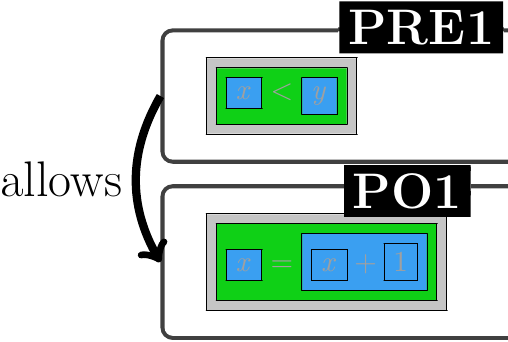
\includegraphics[scale=0.2]{Figures/Formalising/dra1.png}}
      &  
\raisebox{-\totalheight}{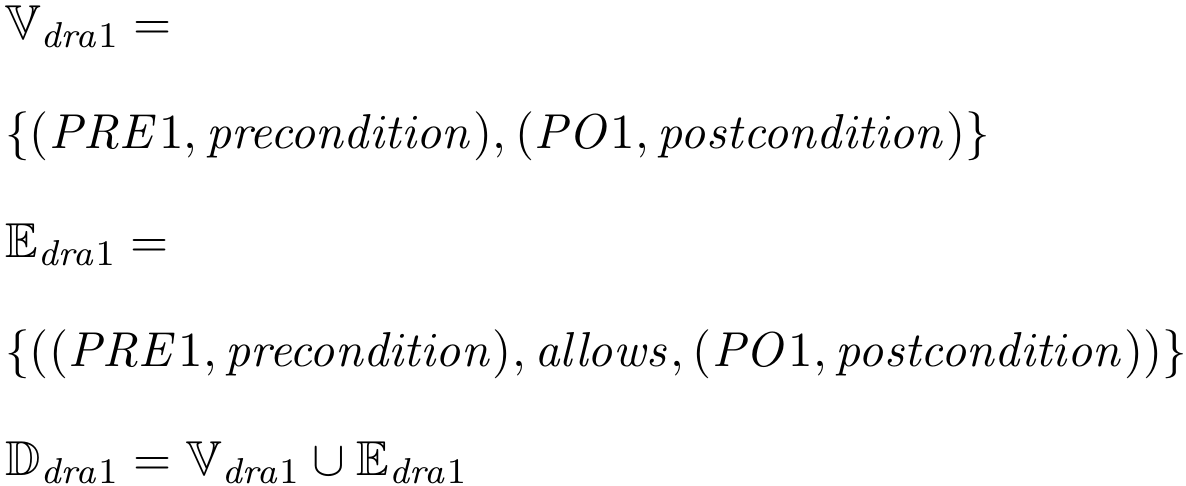
\includegraphics[scale=0.2]{Figures/Formalising/dra1txt.png}}
\\ \hline
dra2)
      & 
\raisebox{-\totalheight}{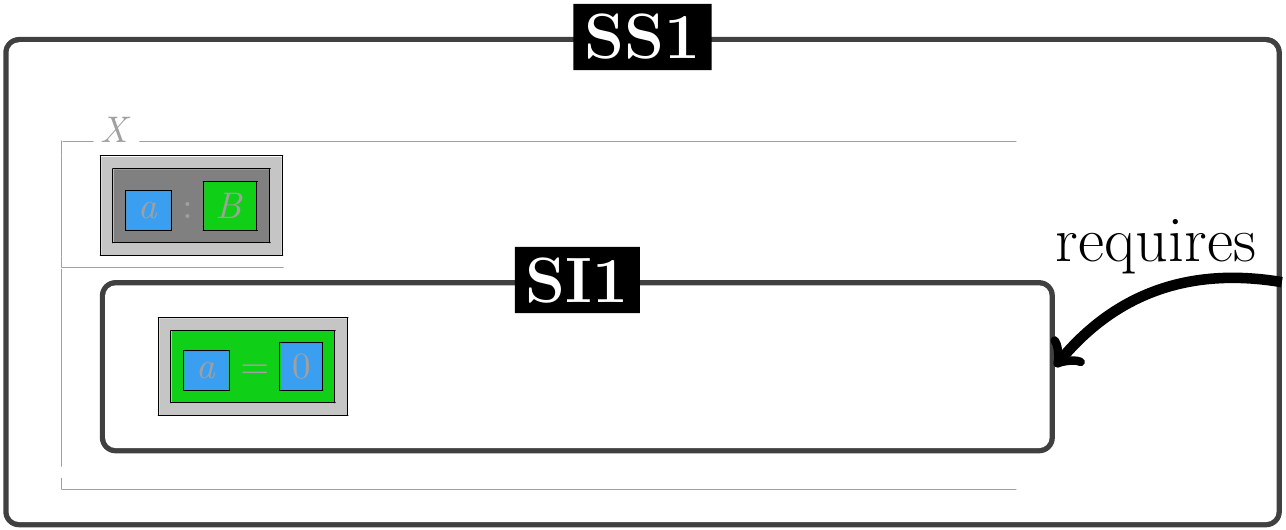
\includegraphics[scale=0.08]{Figures/Formalising/dra2.png}}
      &  
\raisebox{-\totalheight}{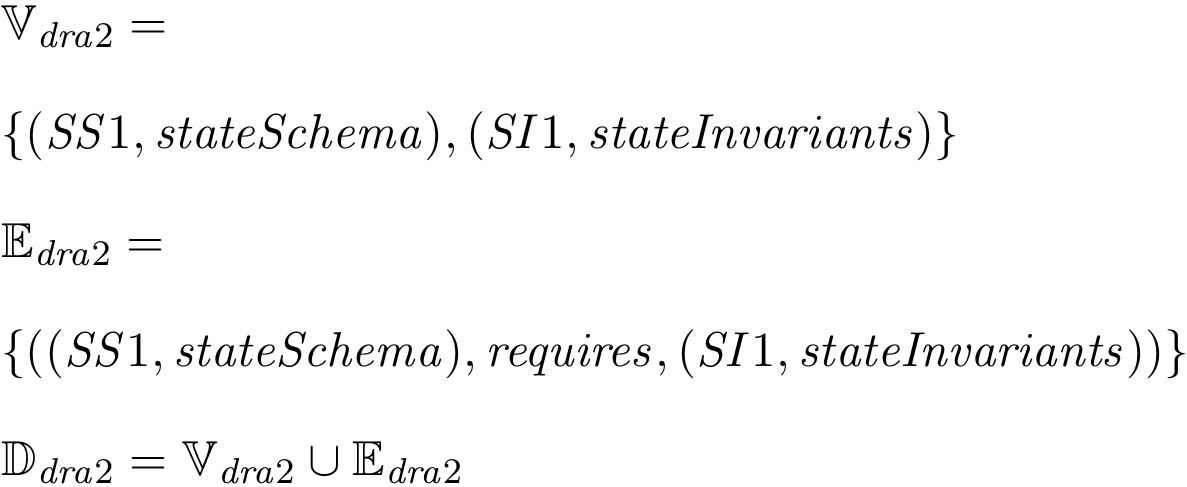
\includegraphics[scale=0.2]{Figures/Formalising/dra2txt.png}}
\\ \hline
dra3)
      & 
\raisebox{-\totalheight}{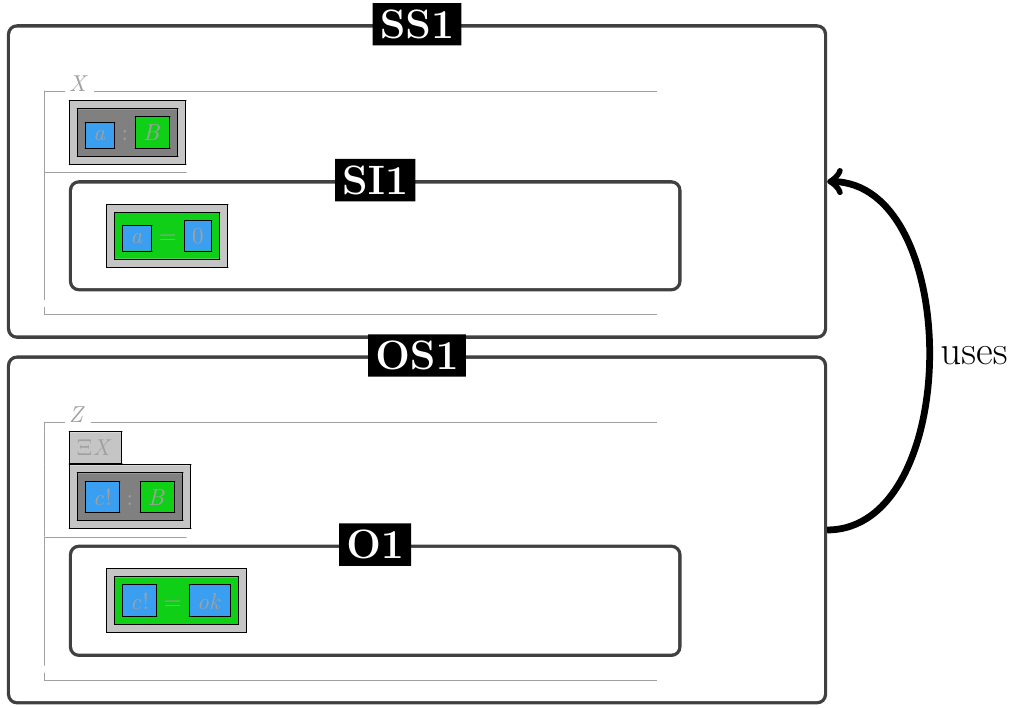
\includegraphics[scale=0.1]{Figures/Formalising/dra3.png}}
      &  
\raisebox{-\totalheight}{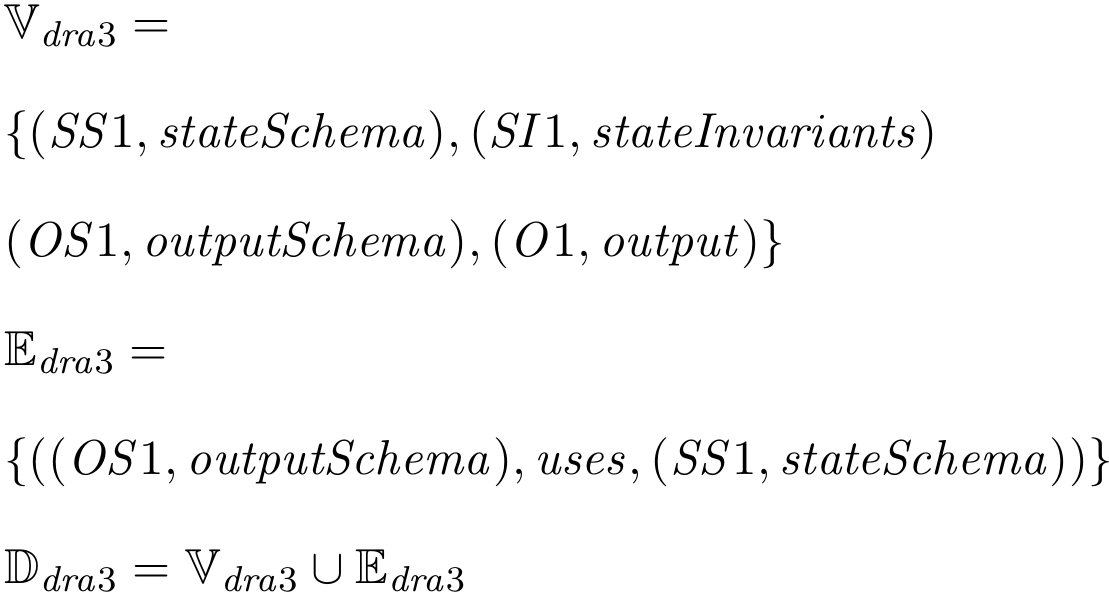
\includegraphics[scale=0.2]{Figures/Formalising/dra3txt.png}}
\\ \hline
dra4)
      & 
\raisebox{-\totalheight}{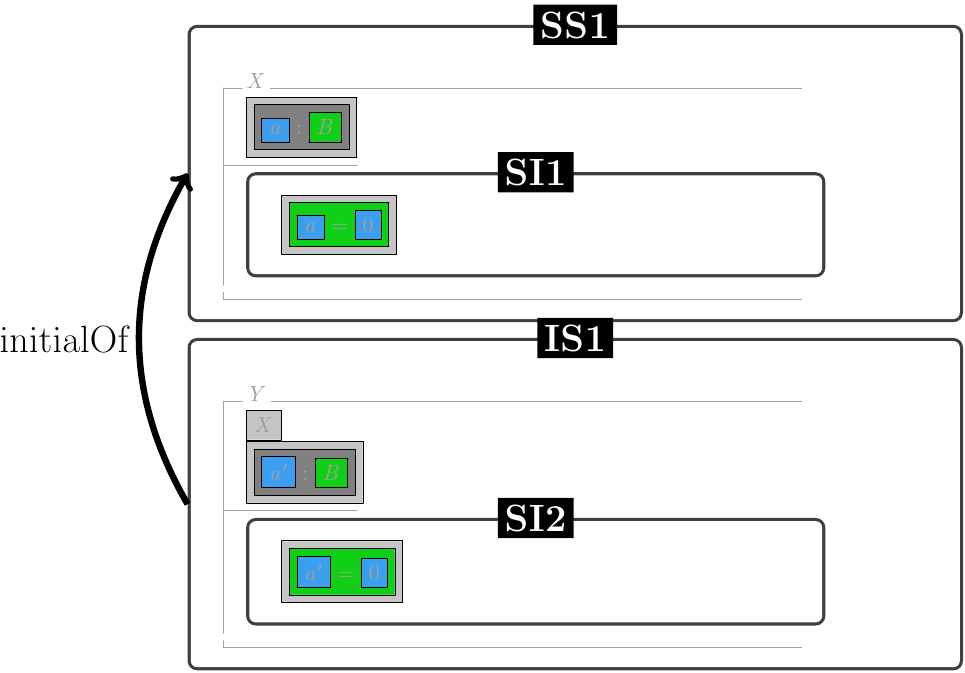
\includegraphics[scale=0.1]{Figures/Formalising/dra4.png}}
      &  
\raisebox{-\totalheight}{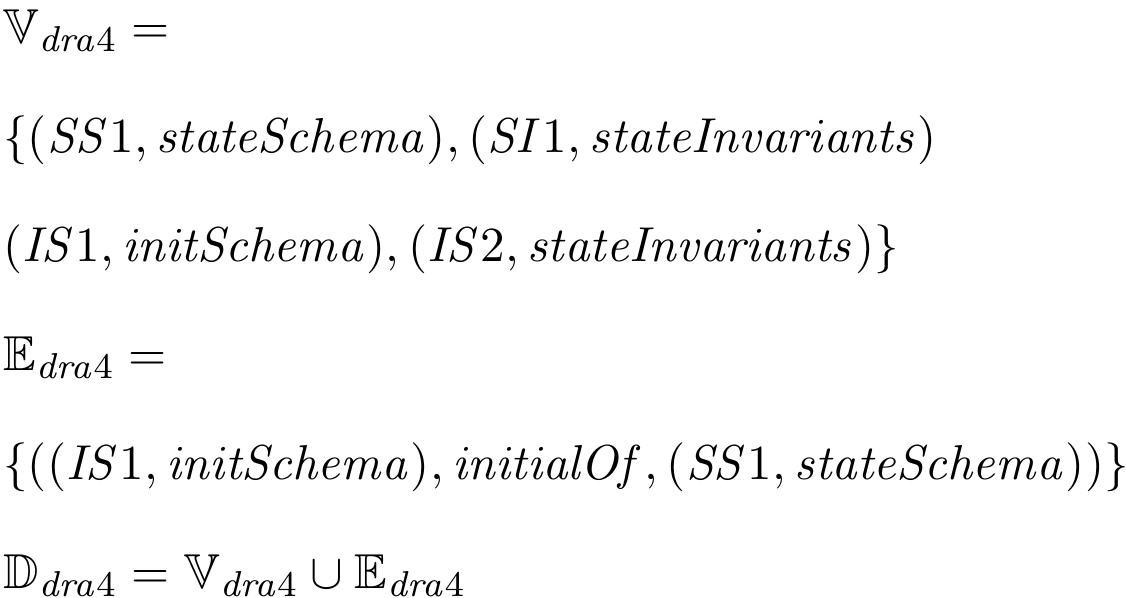
\includegraphics[scale=0.2]{Figures/Formalising/dra4txt.png}}
\\ \hline
dra5)
      & 
\raisebox{-\totalheight}{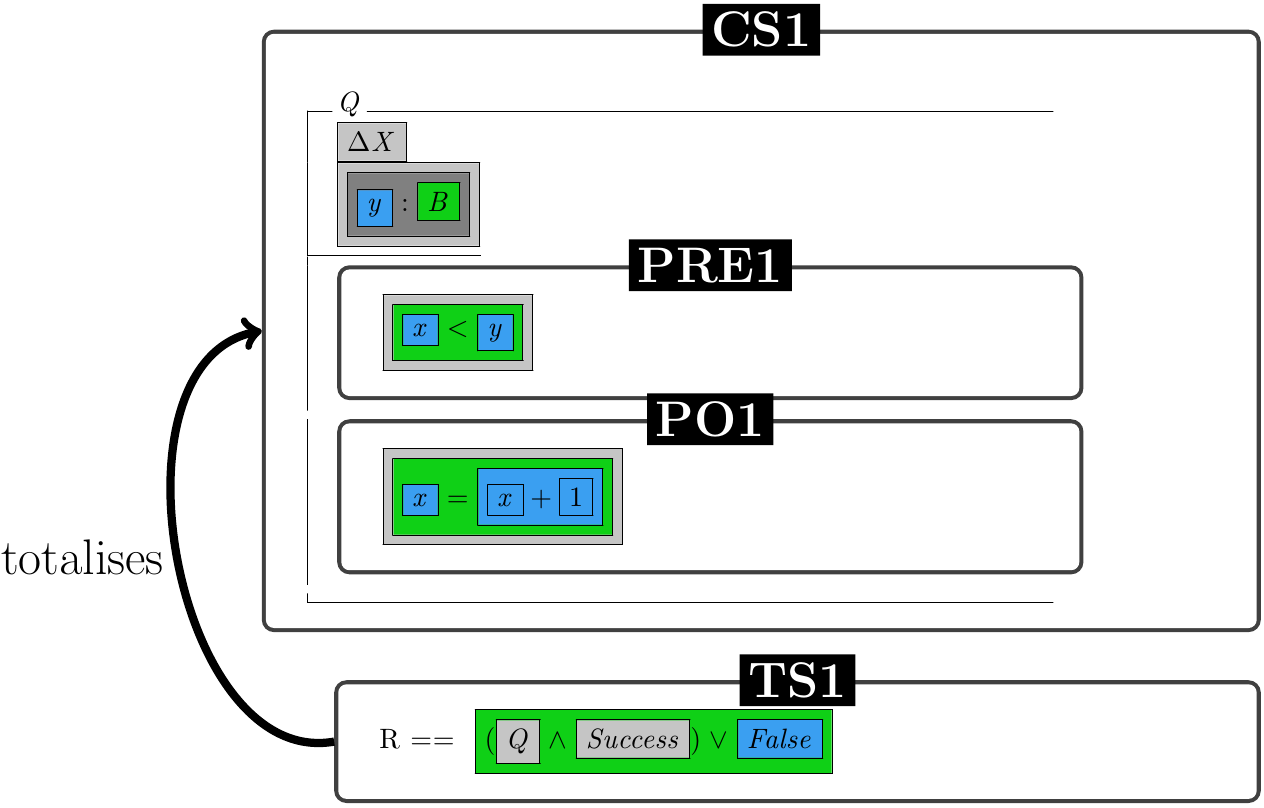
\includegraphics[scale=0.1]{Figures/Formalising/dra5.png}}
      &  
\raisebox{-\totalheight}{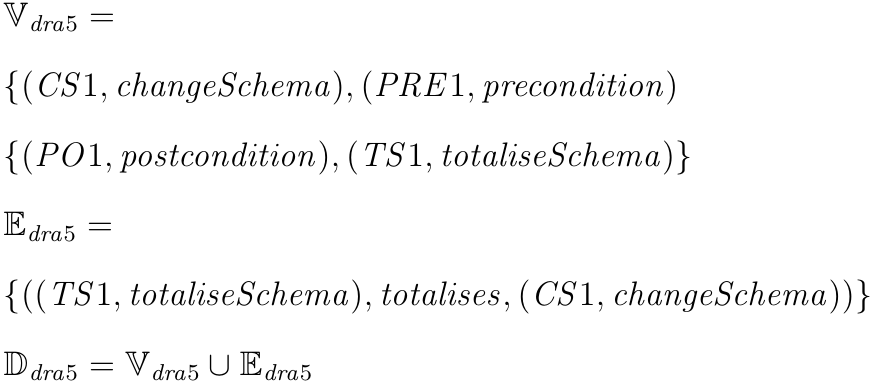
\includegraphics[scale=0.3]{Figures/Formalising/dra5txt.png}}
\\ \hline
\end{tabular}
\caption{Using the formalised definitions for vertices and edges to create a dependency graph. \label{tab:verticiesandedges}}
\end{center}
\end{table}

%\begin{tabular}{l l l}
% & & $\mathbb{V}_{dra5} =$ \\
%& & $\{(CS1, changeSchema), (PRE1, precondition)$\\
%& & $\{(PO1, postcondition), (TS1, totaliseSchema)\}$\\
% & & $\mathbb{E}_{dra5} =$ \\
% & & $\{((TS1, totaliseSchema), totalises, (CS1, changeSchema))\}$ \\
% & & $\mathbb{D}_{dra5} = \mathbb{V}_{dra5} \union \mathbb{E}_{dra5}$ \\
%\end{tabular}

Table \ref{tab:verticiesandedges} show how a dependency graph can be created using the formal definitions for vertices and edges. The dependency graph is directly generated from the \gls{zdra} annotated document. The relations \emph{intialOf} and \emph{uses} are used between schemas, \emph{requires} becomes a childOf the schema which requires it and \emph{allows} can be used between instances within the schema (see table \ref{tab:relationsallowed}). If the \emph{allows} relationship is used within the schema, then both the precondition and postcondition/output becomes childrenOf the schema. Figure \ref{fig:unnested} shows two separate schemas which are not nested within eachother, however figure \ref{fig:nested} shows the precondition PRE2 allows the postcondition PO2 within the schema CS1, since CS1 requires PRE2 then both PRE2 and PO2 are chidrenOf CS1.

\begin{figure}[H]
\centering
\begin{minipage}{0.45\textwidth}
\centering
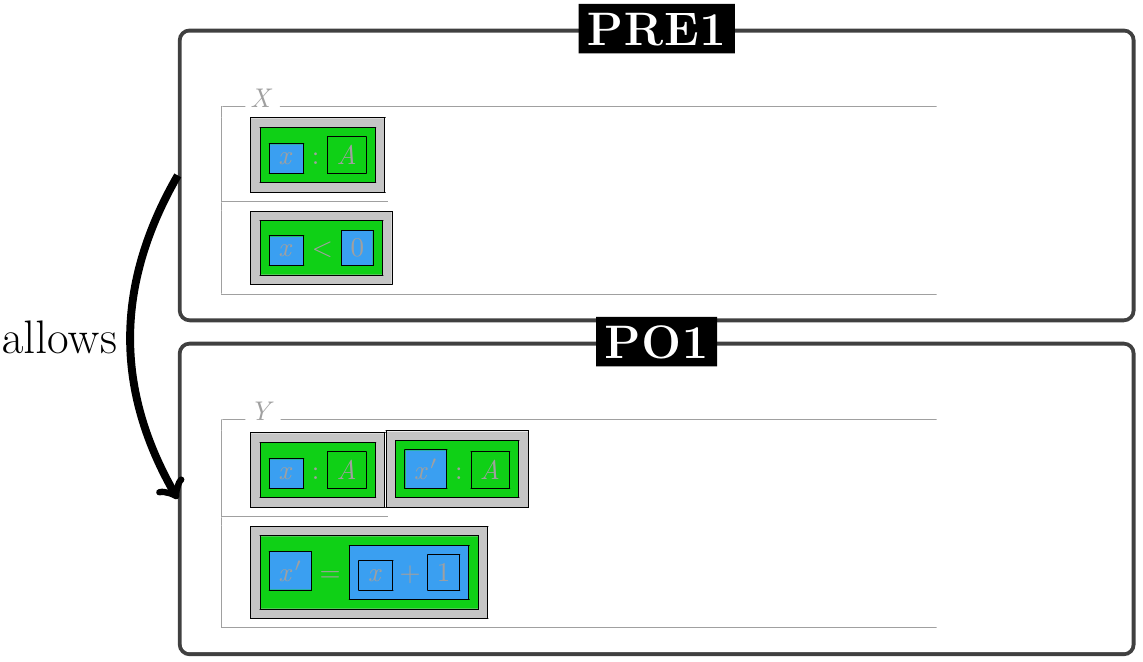
\includegraphics[scale=0.18]{Figures/Formalising/unnested.png}
\caption{Relation with un-nested precondition and postcondition.  \label{fig:unnested}}
\end{minipage}\hfill
\begin{minipage}{0.45\textwidth}
\centering
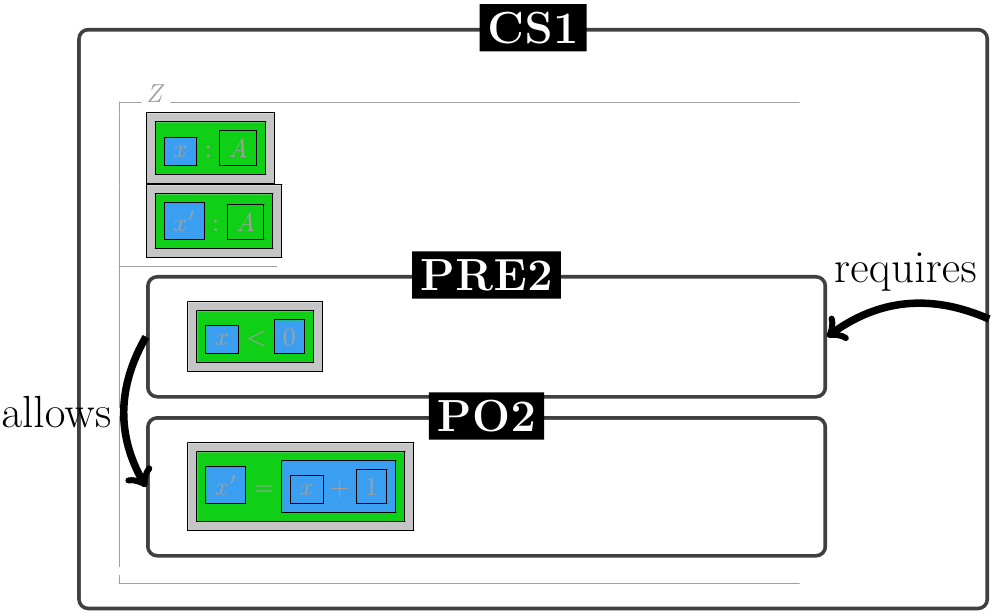
\includegraphics[scale=0.18]{Figures/Formalising/nested.png}
\caption{Relation with nested precondition and postcondition.  \label{fig:nested}}
\end{minipage}
\end{figure}

If we combine all the annotations in table \ref{tab:verticiesandedges} (whilst adding PRE1 and PO1 in a schema named CS1) we get a fully annotated specification and its dependency graph shown in figure \ref{fig:draspec} and \ref{fig:draspecdep} respectively.

\begin{figure}[H]
\centering
\begin{minipage}{0.45\textwidth}
\centering
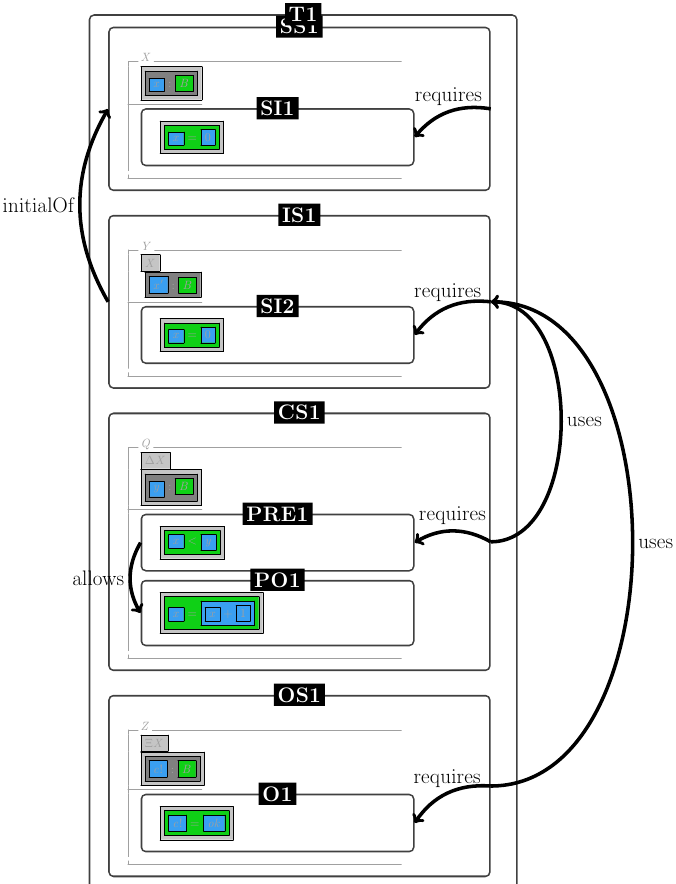
\includegraphics[scale=0.18]{Figures/Formalising/draspec.png}
\caption{All annotations from table \ref{tab:verticiesandedges} combined into one specification.  \label{fig:draspec}}
\end{minipage}\hfill
\begin{minipage}{0.5\textwidth}
\centering
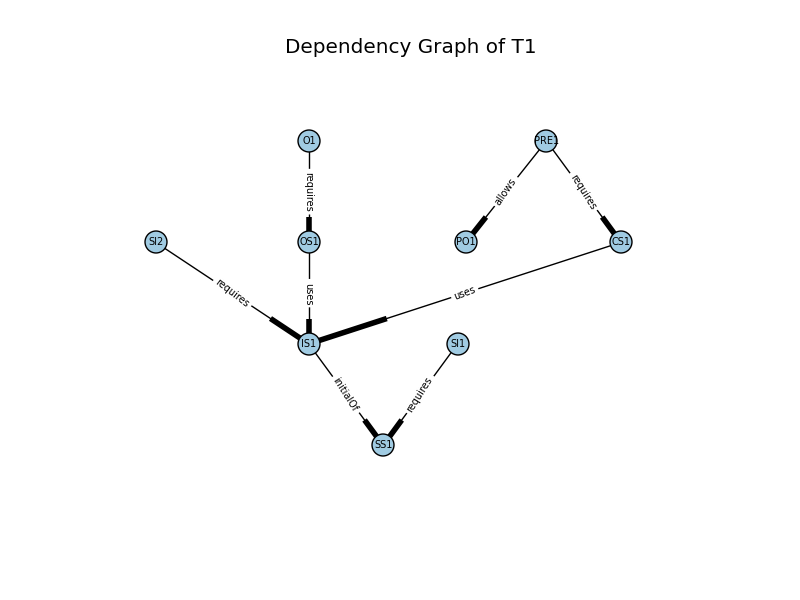
\includegraphics[scale=0.5]{Figures/Formalising/dp_text.png}
\vspace{-1.1in}
\caption{Dependency graph of the example in \ref{fig:draspec} \label{fig:draspecdep}}
\end{minipage}
\end{figure}

\noindent Since figure \ref{fig:draspec} is a combination of the annotations in table \ref{tab:verticiesandedges} we can call this dependency graph $\mathbb{D}_{comb}$ where \newline $\mathbb{V}_{comb} = \{ \\
(T1, theory),(SS1, stateSchema), (SI1, stateInvariants), \\ (IS1, initSchema), (SI2, stateInvariants), (CS1, changeSchema), \\ (PRE1, precondition), (PO1, postcondition), (OS1, outputSchema), (O1, output)
\}$
\newline
\noindent and $\mathbb{E}_{comb} = \{ \\
((SS1, stateSchema), requires, (SI1, stateInvariants)) \\
((IS1, initSchema), requires, (SI2, stateInvariants)) \\
((IS1, initSchema), initialOf, (SS1, stateSchema)) \\
((CS1, changeSchema), requires, (PRE1, precondition)) \\
((PRE1, precondition), allows, (PO1, postcondition)) \\
((CS1, changeSchema), uses, (IS1, initSchema)) \\
((OS1, outputSchema), requires, (O1, output)) \\
((OS1, outputSchema), uses, (SS1, stateSchema)) \\
\}
$
\newline
\noindent and $\mathbb{D}_{comb} = \mathbb{V}_{comb} \union \mathbb{E}_{comb}$

\begin{defin}
The function anns(s) returns all annotations ann within a draschema. Thus:
\begin{figure}[H]
\centering
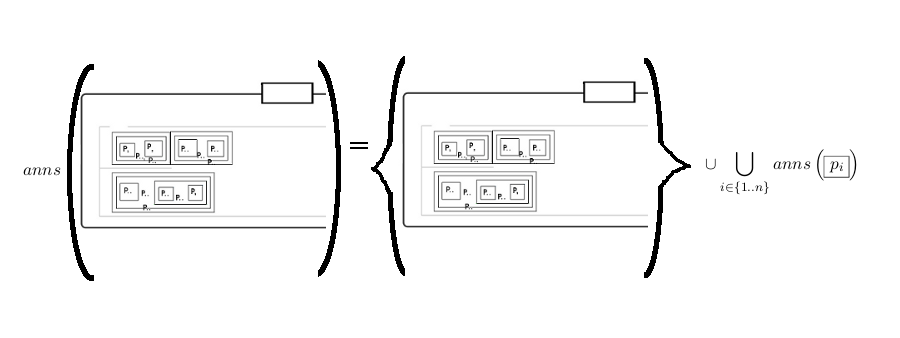
\includegraphics[scale=0.45]{Figures/Formalising/anns2.png}
\end{figure}
\end{defin}

We have a definition for the function \emph{anns(s)} which returns all the \gls{zcga} annotations for a vertex in a graph.

\begin{defin}
\textbf{(First child of an annotation}) For an annotation 

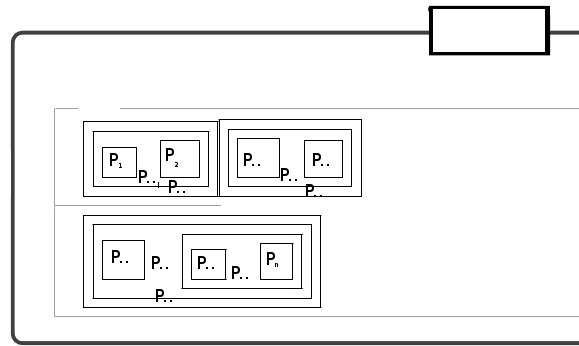
\includegraphics[scale=0.3]{Figures/Formalising/anns.png}

we introduce the function first(ann):

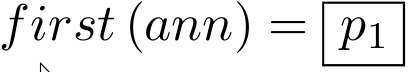
\includegraphics[scale=0.2]{Figures/Formalising/firstann2.png}

\end{defin}

\begin{figure}[H]
\centering
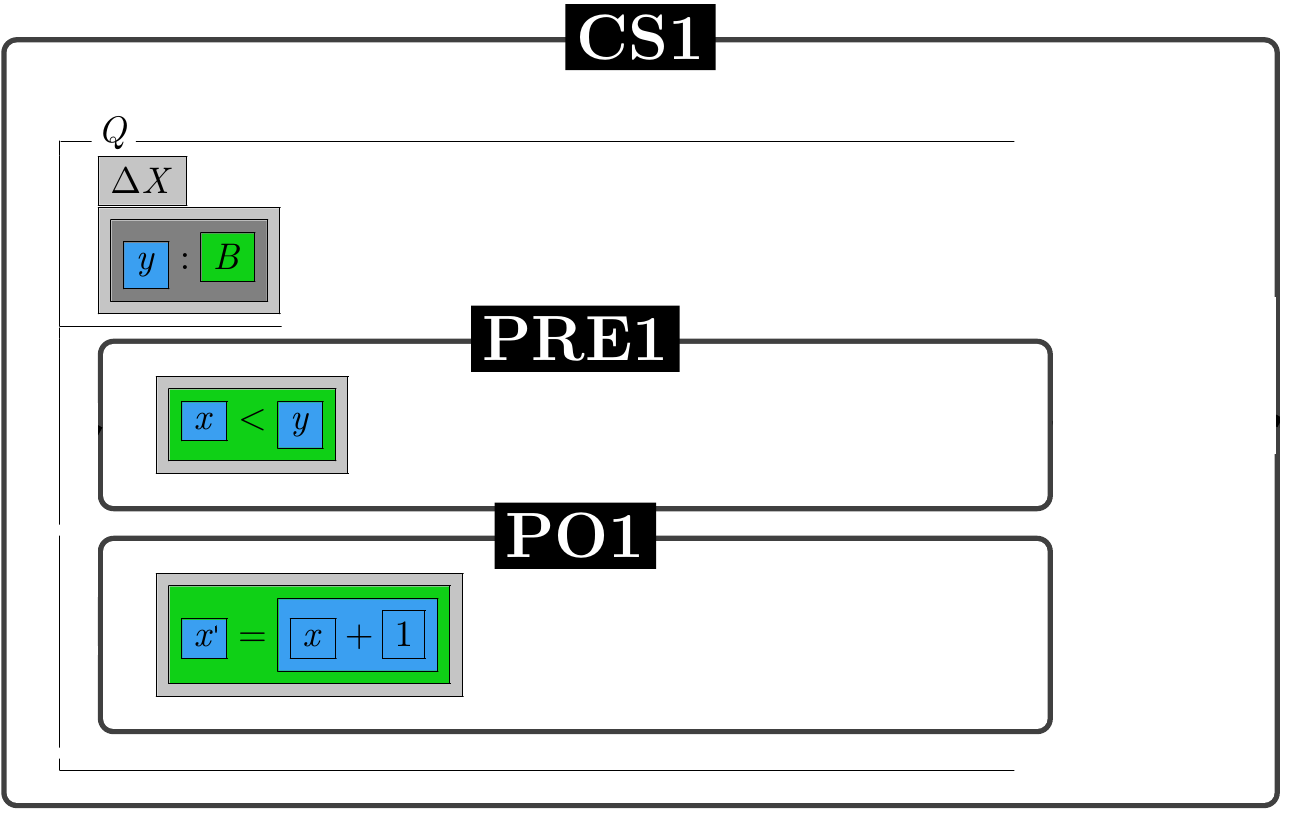
\includegraphics[scale=0.15]{Figures/Formalising/exampleschema.png}
\caption{Example of a draschema fully annotated in \gls{zcga} and \gls{zdra} \label{fig:draschemaanns}}
\end{figure}

\begin{table}[H]
\begin{tabular}{|l | l | l |}
\hline
\textbf{Set} & \textbf{Description} & \textbf{Example for} \\
& & \textbf{figure \ref{fig:draschemaanns}} \\
\hline
$\mathtt{T}(v)$ & $\{\mathbf{R}(x)| x \in anns(s) \land role(x) = \mathbf{term}\}$ & $\{y, x, 1\}$ \\
\hline
$\mathtt{S}(v)$ & $\{\mathbf{R}(x)| x \in anns(s) \land role(x) = \mathbf{set}\}$ & \{\} \\
\hline
$\mathtt{P}(v)$ & $\{\mathbf{R}(x)| x \in anns(s) \land role(x) = \mathbf{expression}\}$ & $\{B, lessthan(x, y)$ \\
& & $equal(x',plus(x,1)) \}$\\
\hline
$\mathtt{DC}(v)$ & $\{inter(first(x))| x \in anns(s) \land role(x) = \mathbf{dec}\}$ & $\{y\}$ \\
\hline
$\mathtt{DF}(v)$ & $\{inter(first(x))| c \in anns(s) \land role(x) = \mathbf{def}\}$ & $\{\}$ \\
\hline
$\mathtt{ST}(v)$ & $\{\mathbf{R}(x)| x \in anns(s) \land role(x) = \mathbf{schematext}\}$ & $\{y:B,$ \\
& & $lessthan(x,y),$ \\
& & $equal(x',plus(x,1)) \}$ \\
\hline
$\mathtt{ENV}(v)$ & $\{\mathbf{R}(x) | \exists v' \neq v$ with $v'$ is a vertex in the & \\
& preorder path from the root vertex to vertex $v$ & \\
& and $x \in anns(v') \land role(x) = expression\}$ & \\
\hline
\end{tabular}
\caption{ Sets for a node $v$ and examples. \label{tab:setsfornodes}}
\end{table}

\begin{defin}
\textbf{(Introduced Symbols.)} We define the set $\mathtt{IN}(v)$ of introduced symbols and facts of a node v as follows:

$\mathtt{IN}(v) := \mathtt{DF}(v) \union \mathtt{DC}(v) \union \{s|s \in \mathtt{P}(v) \land s \notin \mathtt{ENV}(v)\} \bigcup\limits_{c\ childOf\ v} \mathtt{IN}(c)$
\end{defin}

\begin{defin}
\textbf{(Used Symbols.)} A node v uses the set $\mathtt{USE}(v)$ is as follows:

$\mathtt{USE}(v) := \mathtt{T}(v) \union \mathtt{S}(v) \union \mathtt{P}(v) \bigcup\limits_{c\ childOf\ v} \mathtt{USE}(c)$
\end{defin}

With our new definitions for symbols and facts along with table \ref{tab:setsfornodes} showing the available sets in a node we can prove some properties about the nodes in the dependency graph.

\begin{thm}
\label{dfdcvertex}
$\mathtt{DF}(v) \union \mathtt{DC}(v) \subseteq \mathtt{T}(v) \union \mathtt{S}(v)$ for each vertex v.
\end{thm}

\begin{proof}
By using table \ref{tab:setsfornodes}, $\mathtt{DF}(v)$ and $\mathtt{DC}(v)$ only ontain the first children of the defintion and declarations of the annotations. Thus by the definition of first child of annotation and the \gls{zcga} weak types in chapter \ref{chap:zcga} the only children can be of type \texttt{term} or \texttt{set} and are therefore in the sets $\mathtt{T}(v)$ or $\mathtt{S}(v)$ respectively.
\end{proof}

\begin{thm}
\label{insubsetuse}
$\mathtt{IN}(v) \subseteq \mathtt{USE}(v)$ in each node v.
\end{thm}

\begin{proof}
In theorem \ref{insubsetuse} we have two scenarios to consider:

\begin{itemize}
\item If $v$ have no children then use theorem \ref{dfdcvertex}.

\item If $v$ has children then by assume the theorem holds for all children $c$ of $v$ then by theorem \ref{dfdcvertex} and the induction hypothesis it is true that $\mathtt{IN}(v) \subseteq \mathtt{USE}(v)$
\end{itemize}
\end{proof}


\subsection{Conclusion}

In this section we have looked at the dependency graph and defined it formally using sets. We have defined the nodes of a graph as a pair and the edges as a triple. We have given examples of certain annotations and how they would be represented formally. Although the dependency graph helps to see the relationships between instances we then need to order them correctly in order to input the specification into a theorem prover. To do this we need to determine the \emph{textual order} of the relations. The textual order of relations is described in the next section.

\section{Generation of the GoTo graph}

Since the dependency graph only follows the annotations of the \gls{zdra} we need to highlight the textual order of these annotations. For example some annotations may be stronger then others. The order in which instances are inputted in the theorem prover are also important so that the theorem prover may be parsed correctly. The GoTo graph is generated using the textual order of the dependency graph.

\begin{defin}[Textual order]
We can now formalise three different kinds of textual order when translating a dependency graph into the GoTo graph.

\begin{itemize}
\item \textbf{Strong textual order $\prec$:} This order describes an entire entity relation between two nodes ($id_{A}$ uses $id_{B}$ would be written as $id_{B}$ $\prec$ $id_{A}$, $id_{A}$ initialOf $id_{B}$ would be written as $id_{B} \prec id_{A}$, $id_{A}$ totalises $id_{B}$ would be written as $id_{B}$ $\prec$ $id_{A}$).

\item \textbf{Weak textual order $\preceq$:} This order describes a sub-part relation between two nodes ($id_{A}$ allows $id_{B}$ within a schema written as $id_{A} \preceq id_{B}$).

\item \textbf{Common textual order $\leftrightarrow$:} This order describes a relation between two nodes where they are both dependent on each other (Where a draschema $id_{A}$ requires a draline of some sort $id_{B}$ is written as $id_{A}$ $\leftrightarrow$ $id_{B}$).
\end{itemize}
\end{defin}

The dependency graph is a direct representation of the \gls{zdra} annotations and arrows represented when compiling the \gls{zdra} annotated document. The GoTo uses these annotations and describes the textual order of them. When inputting a specification into an automatic theorem prover, the textual order is important as it decides which part of the specification needs to be in-putted first in order to parse correctly.

\begin{table}[H]
\centering
\begin{tabular}{| l | l | l |}
\hline
\textbf{Relation} & \textbf{Meaning} & \textbf{Order} \\
\hline 
$id_{A}$, initialOf, $id_{B}$ & $id_{A}$ is the initial schema of $id_{B}$ & $id_{B} \prec id_{A}$ \\
 & or $id_{A}$ initialises $id_{B}$ & \\
 \hline
$id_{A}$, uses, $id_{B}$ & $id_{B}$ is being used in $id_{A}$ & $id_{B} \prec id_{A}$ \\
& or $id_{B}$ is needed in $id_{A}$ & \\
 \hline
 $id_{A}$, totalises, $id_{B}$ & $id_{A}$ makes the precondition in $id_{B}$ total & $id_{B} \prec id_{A}$ \\
 \hline
$id_{A}$, allows, $id_{B}$ & $id_{A}$ is allowing $id_{B}$ to occus & $id_{A} \preceq id_{B}$ \\
\hline
$id_{A}$, requires, $id_{B}$ & $id_{A}$ is requiring $id_{B}$ to function & $id_{A} \leftrightarrow id_{B}$ \\
\hline
\end{tabular}
\caption{Example of ZDRa annotations and the textual order of them. \label{tab:texorder}}
\end{table}

\begin{defin}
We denote v\_1 and v\_2 to describe node 1 and node 2 respectively for example if we have $\backslash initialof\{id_{1}\}\{id_{2}\}$ and $id_{1}$ is IS1 and $id_{2}$ is SS1 then v\_1 would be (IS1, initialSchema) and v\_2 would be (SS1, stateSchema).
\end{defin}

\begin{algorithm}[H]
\underline{goto\_graph = directedGraph} \;
\underline{dependency\_graph = directedGraph} \;
\SetAlgoLined
\uIf{$\backslash$initialof\{$id_{1}$\}\{$id_{2}$\}} 
{
addEdge(v\_1, $\rightarrow$, v\_2) to dependency\_graph \;
addEdge(v\_2, $\rightarrow$, v\_1)  to goto\_graph\;
}
\uIf{$\backslash$uses\{$id_{1}$\}\{$id_{2}$\}} 
{
addEdge(v\_1, $\rightarrow$, v\_2) to dependency\_graph \;
addEdge(v\_2, $\rightarrow$, v\_1)  to goto\_graph \;
}
\uIf{$\backslash$allows\{$id_{1}$\}\{$id_{2}$\}} 
{
addEdge(v\_1, $\rightarrow$, v\_2) to dependency\_graph \;
addEdge(v\_1, $\rightarrow$, v\_2)  to goto\_graph \;
}
\uIf{$\backslash$requires\{$id_{1}$\}\{$id_{2}$\}} 
{
addEdge(v\_1, $\rightarrow$, v\_2) to dependency\_graph \;
addEdge(v\_1, $\rightarrow$, v\_2)  to goto\_graph \;
}
\uIf{$\backslash$totalises\{$id_{1}$\}\{$id_{2}$\}} 
{
addEdge(v\_1, $\rightarrow$, v\_2) to dependency\_graph \;
addEdge(v\_2, $\rightarrow$, v\_1)  to goto\_graph \;
}
\caption{Algorithm to generate the dependency graph and goto. \label{alg:gotodep} }
\end{algorithm}
\vspace{0.2in}


Algorithm \ref{alg:gotodep} shows the pseudocode of the implementation on how the dependency graph and goto graphs are created. It reads the labels created by the user when annotating the formal specification. 

Note the edges for the relations \emph{allows} and \emph{requires} have the same direction both in the dependency graph and the goto graph. This is because if instance v\_1 \emph{allows} another instance v\_2 to happen then instance v\_1 must exist for instance v\_2 to exist. The relationship \emph{requires} is between a drashchema and a draline where a draschema requires a particular draline, in the algorithm we have the dependency graph edge and goto graph edge point in the same direction.

With the edges for relations \emph{initialof}, \emph{uses} and \emph{totalises}, algorithm \ref{alg:gotodep} changes the direction of the edges from the dependency graph to the goto graph. If a node v\_1 is the initialOf another node v\_2 then v\_1 initialises v\_2, therefore v\_2 must exist first for v\_1 to initialise it. If a node v\_1 uses another node v\_2 then v\_2 must exist first before it can be used by v\_1. This is the same with the relation \emph{totalises}, if a node v\_1 totalises another node v\_2 then the node v\_2 must exist before the node v\_1 can totalise it.

\begin{figure}[H]
\centering
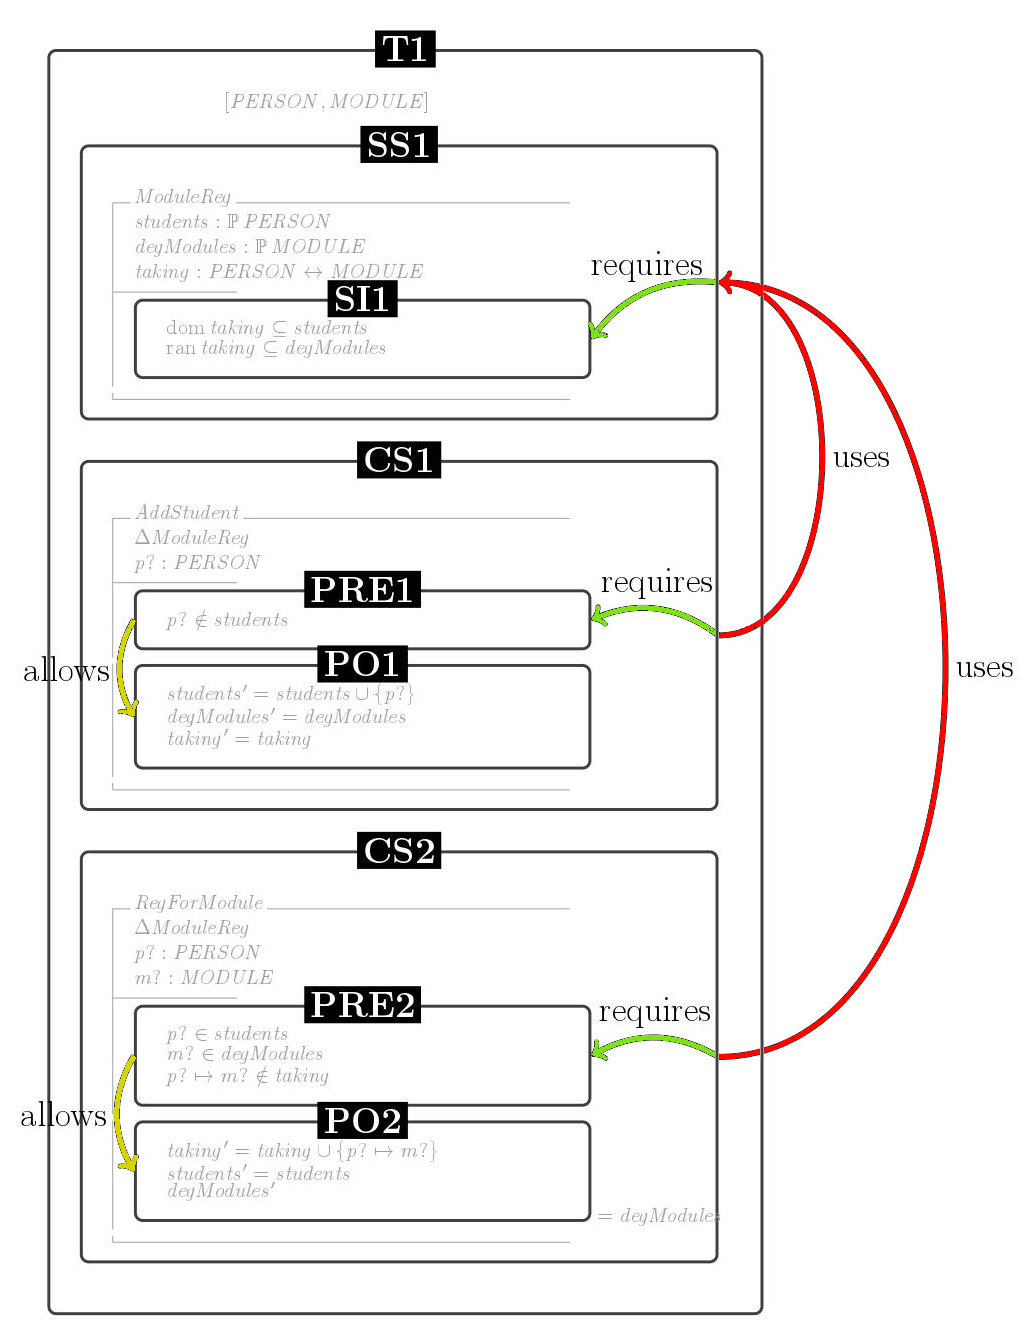
\includegraphics[scale=0.55]{Figures/Formalising/dramodule.png}
\caption{User annotated in \gls{zdra} for the modulereg specification with arrows coloured. \label{fig:zdramodule}}
\end{figure}

\begin{figure}[H]
\centering
\begin{minipage}{0.47\textwidth}
\centering
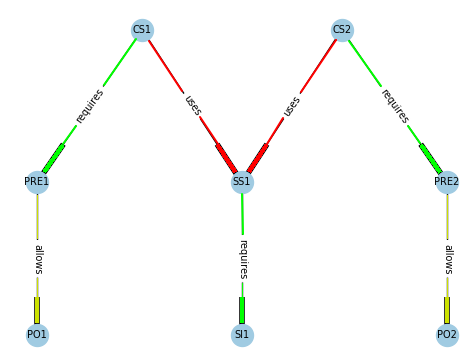
\includegraphics[scale=0.55]{Figures/Formalising/dpmodule.png}
\caption{The dependency graph of modulereg specification with arrows coloured.  \label{fig:dpmodule}}
\end{minipage}\hfill
\begin{minipage}{0.47\textwidth}
\centering
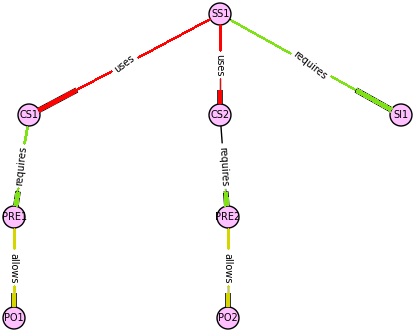
\includegraphics[scale=0.55]{Figures/Formalising/gotomodule.png}
\caption{The goto graph of modulereg specification with arrows coloured. \label{fig:gotomodule}}
\end{minipage}
\end{figure}

Figure \ref{fig:zdramodule} shows the moduleReg specification annotated in \gls{zdra} however the colours of the arrows have been changed as to compare it with the automatically generated dependency graph (figure \ref{fig:dpmodule}) and it's corresponding goto grah (figure \ref{fig:gotomodule}). Note the red arrows which correspond to the `uses' relation are facing the same direction in the user annotated document and in the dependency graph (from CS1 to SS1 and from CS2 to SS1) however they go the opposite direction in the goto graph. This goes the same for the green arrows which represent the `requires' relation. On the other hand the yellow arrow, representing the `allows' relation goes in the same direction in all three figures.

\subsection{Conclusion}

In this section we have highlighted why the goto grph is important and divded the \gls{zdra} annotations into their correctly textual ordered categories (strong, weak and common). We added an algorithm to this section to describe how the dependency graph and goto graph are created from the \gls{zdra} annotations inputted by the user. We also compared the \gls{zdra} annotated specification and its corresponding dependency and goto graphs in more detail and shown which arrows change direction in practice. In the next section we take a formal look at the the goto graph.

\section{Formal View on the GoTo Graph}

\begin{defin}[Textual order edge]
We can say a textual order edge $\mathbb{O}$ is a quadruple
\begin{center}
($v_{A}, v_{B}, rel, to$)
\end{center}
where it is a relation rel, from node $v_{A}$ to node $v_{B}$ and it's textual order to where $to \in \{\prec , \preceq , \leftrightarrow , \succ , \succeq \}$.
\end{defin}

\begin{defin}[Graph of Textual order]
A graph of textual order is a pair (V,O), made up of a set of vertices V and a set of ordered edges O.
\end{defin}

The main reason for producing a GoTo graph is to automatically produce a skeleton for a certain theorem prover.

\begin{table}[H]
\centering
\begin{tabular}{| c | c | c |}
\hline
\textbf{Relation} & \textbf{Textual} & \textbf{GoTo} \\
& \textbf{Order} & \textbf{Edge} \\
\hline
($v_{A}$, uses, $v_{B}$) & $v_{A} \succ v_{B}$ & 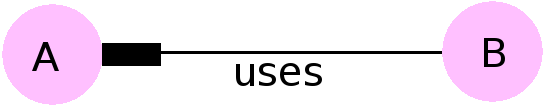
\includegraphics[scale=0.15]{Figures/Formalising/uses.png} \\
\hline
($v_{A}$, initialof, $v_{B}$) & $v_{A} \succ v_{B}$  & 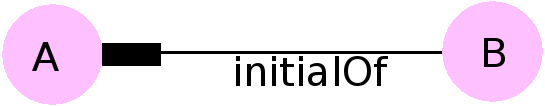
\includegraphics[scale=0.15]{Figures/Formalising/initialof.png} \\
\hline
($v_{A}$, allows, $v_{B}$) & $v_{A} \preceq v_{B}$ & 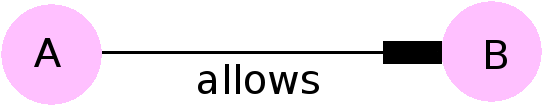
\includegraphics[scale=0.15]{Figures/Formalising/allows.png} \\
\hline
($v_{A}$, totalises, $v_{B}$) & $v_{A} \succ v_{B}$ & 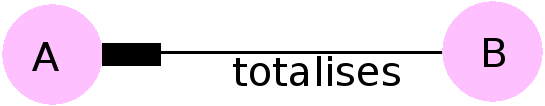
\includegraphics[scale=0.15]{Figures/Formalising/totalises.png} \\
\hline
($v_{A}$, requires, $v_{B}$) & $v_{A} \leftrightarrow v_{B}$ & 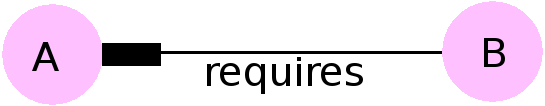
\includegraphics[scale=0.15]{Figures/Formalising/requires.png} \\
\hline
\end{tabular}
\caption{The relations representedby textual order and in the goto graph \label{tab:gotorelations}}
\end{table}

Table \ref{tab:gotorelations} shows what the textual order reprsentation of each relation is and how it is represented as an edge in the GoTo graph. The uses relation has the texutal order `$\succ$' where the goto graph edge would be $(v_{A}, v_{B}, uses, \succ)$ as the relation uses would have a strong textual order. the initialof relation is similar to the uses relation where the syntax in the goto graph would be $(v_{A}, v_{B}, initialof, \succ)$. Totalises relation also has a similar edge to uses and initialof as the syntax for the goto graph edge would be: $(v_{A}, v_{B}, totalises, \succ)$. The allows relation has a weak textual order where the goto edge syntax would be $(v_{A}, v_{B}, allows, \preceq)$. The requires relation uses the textual symbol `$\leftrightarrow$' as the requires describes a relation that is $subpart\ of$, for example if we have $v_{A}$, requires, $v_{B}$ then this describes a relation that $v_{A}$ is $subpart\ of$ $v_{B}$ therefore the goto edge syntax would be $(v_{A}, v_{B}, requires, \leftrightarrow)$.

\begin{figure}[H]
\centering
\begin{minipage}{0.35\textwidth}
\centering
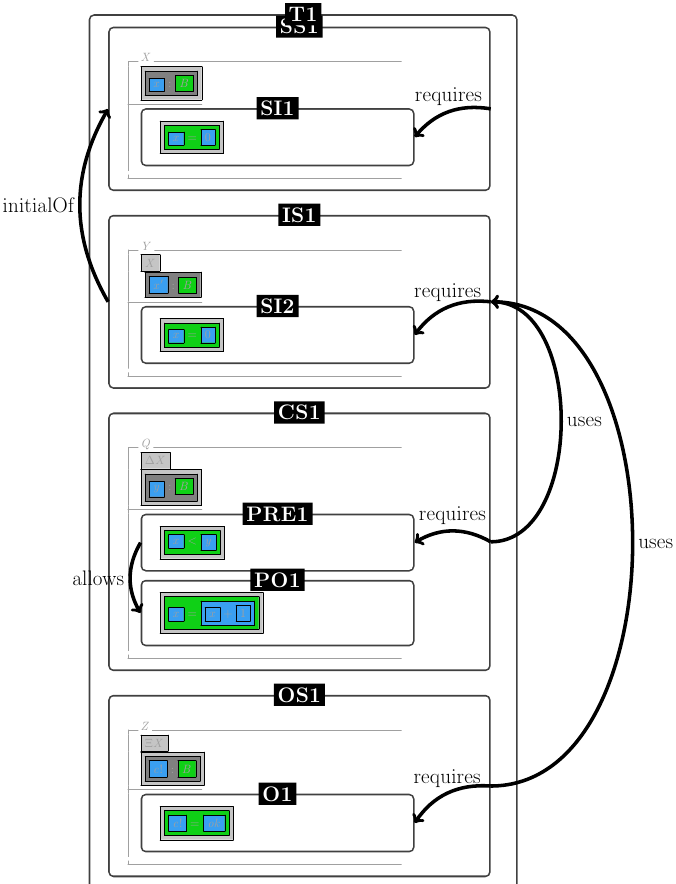
\includegraphics[scale=0.18]{Figures/Formalising/draspec.png}
\caption{All annotations from table \ref{tab:verticiesandedges} combined into one specification.  \label{fig:draspeca}}
\end{minipage}\hfill
\begin{minipage}{0.6\textwidth}
\centering
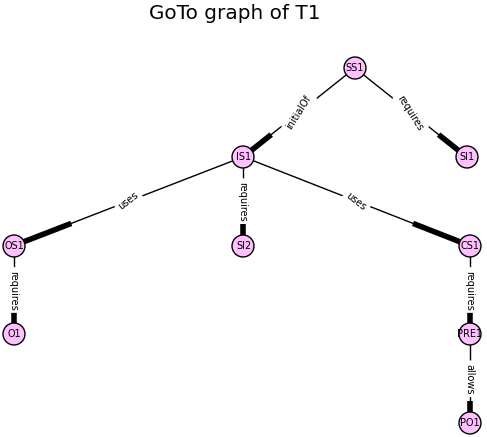
\includegraphics[scale=0.5]{Figures/Formalising/goto_text.png}
\vspace{-1.1in}
\caption{Goto graph of the example in \ref{fig:draspeca} \label{fig:gotospecdep}}
\end{minipage}
\end{figure}

Therefore our nodes would be:

$\mathbb{V}_{figure\ \ref{fig:gotospecdep}}=
\{ \\
(T1, theory),(SS1, stateSchema), (SI1, stateInvariants), \\ (IS1, initSchema), (SI2, stateInvariants), (CS1, changeSchema), \\ (PRE1, precondition), (PO1, postcondition), (OS1, outputSchema), (O1, output)
\}$\\

\noindent and our edges would be: \\
$\mathbb{O}_{figure\ \ref{fig:gotospecdep}}= \{ \\
((SS1, stateSchema), (SI1, stateInvariants), requires, \leftrightarrow) \\
((IS1, initSchema), (SI2, stateInvariants), requires, \leftrightarrow) \\
((IS1, initSchema),  (SS1, stateSchema), initialOf, \succ) \\
((CS1, changeSchema), (PRE1, precondition), requires, \leftrightarrow) \\
((PRE1, precondition), allows, (PO1, postcondition), allows, \preceq) \\
((CS1, changeSchema), (IS1, initSchema), uses, \succ) \\
((OS1, outputSchema), (O1, output), requires, \leftrightarrow) \\
((OS1, outputSchema), (SS1, stateSchema), uses, \succ) \\
\}
$\\

Therefore the goto graph would be the pair $\mathbb{V}_{figure\ \ref{fig:gotospecdep}}, \mathbb{O}_{figure\ \ref{fig:gotospecdep}}$ which we could use to input into a theorem prover.

\subsection{Conclusion}

In this section we took a formal view of the GoTo graph. We have described the edges as a quadruple and defined the graph itself to be a pair. The textual order of each relation has been described and an example has been shown of how to define a goto graph formally.

\section{Chapter Conclusion}

Since the \gls{zcga} has already been touched upon formally via \cite{wtt} it was important to somewhat formally define the \gls{zdra} and graphs produced. This chapter took a formal view on the \gls{zdra} and described the aspect using certain definitions and rules to be followed. Formal properties about the aspect have been highlighted and proved using the definitions and rules defined throughout this thesis. 

The automatically generated dependency graph has also been looked at formally using definitions for the nodes and edges. Examples have been given of formally defined specifications using the definitions highlighted. We took a look at how different symbols and facts are introduced using instances annotated in \gls{zmath}.

The generation of the Goto graph from the dependency graph was illustrated in detail. The textual order of the relations was then described and explained why it was important. Examples were given of dependency graphs and goto graphs to highlight how they varied and the algorithm of the goto and dependency generation was given.

The consecutive chapter highlghted the formalities of the goto graph and gave formal definitions similar to the formal take on the dependency graph. The relations were given certain rules to follow to describe the textual order of them and then an example was given. 

In the next chapter we take a look at the interface in which a one can use the \gls{zmath} and ultimatly translate a formal/semi formal specification into a theorem prover.


